% Appendix C
\pagebreak
\section{Waspmote Battery Life Analysis}
\label{AppendixD} % For referencing this appendix elsewhere, use 
%--------------------------------------------------------------------
\subsection{High Performance Mode, without ZigBee sleep}
For this calculations it is supposed the batteries are in good condition and can be used with optimal conditions. The time values are taken from the third test scenario discussed in section \ref{second}, meaning that the Waspmote uses \textit{Hibernate} or \textit{Deepsleep} and the XBee is completely disconnected from the network.
The results are shown in figures \ref{fig:batCalcHP}, \ref{fig:batCalcHP1} and table \ref{fig:consump}.\\
%--------------------------------------------------------------------
\begin{figure}[htbp]
\centering
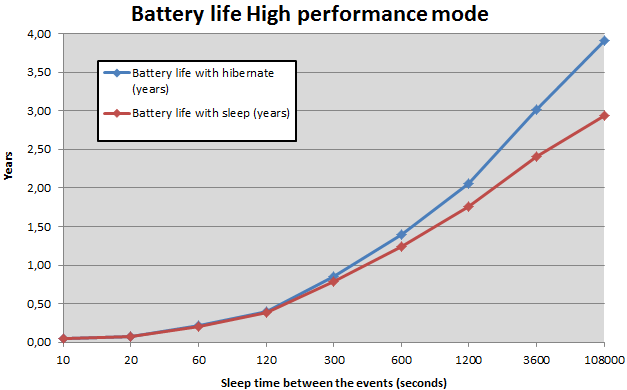
\includegraphics[height=8cm]{batCalcHP}
\caption{Battery life in High performance mode}
\label{fig:batCalcHP}
\end{figure}
%-----------------------------
\begin{figure}[htbp]
\centering
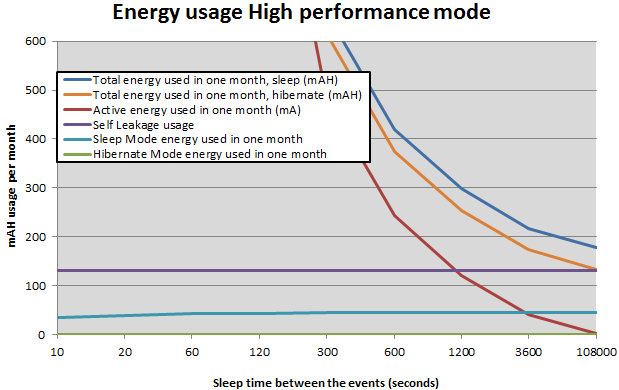
\includegraphics[height=8cm]{battery1}
\caption{Energy usage in High performance mode}
\label{fig:batCalcHP1}
\end{figure}
%-----------------------------
\begin{figure}[htbp]
\centering
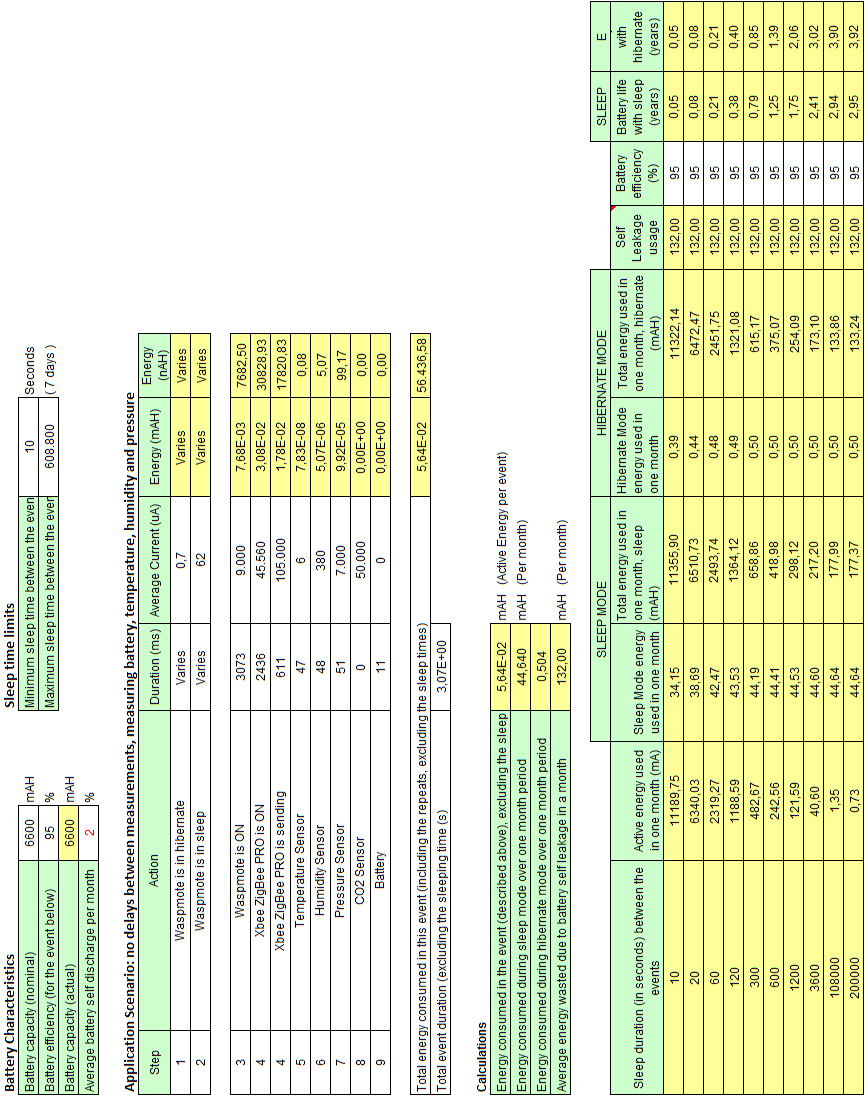
\includegraphics[height=23cm]{cons1}
\caption{Energy usage in High performance mode}
\label{fig:consump}
\end{figure}
\pagebreak
%-------------------------------------------------------------------
\subsection{Power Saver Mode, without ZigBee sleep}
For these calculations Power Saver Mode is supposed. The Waspmote will switch on to measure sensors but not to send the data. The values will only be sent once every 60 samples, saving energy. The results are shown in figures \ref{fig:batCalcPS}, \ref{fig:batCalcPS1} and tables \ref{tab:sendTime3} and \ref{fig:consump2}. Finally table \ref{tab:cons2} summarizes the battery duration in years of both performance and power saver mode.\\
\begin{figure}[!ht]
\centering
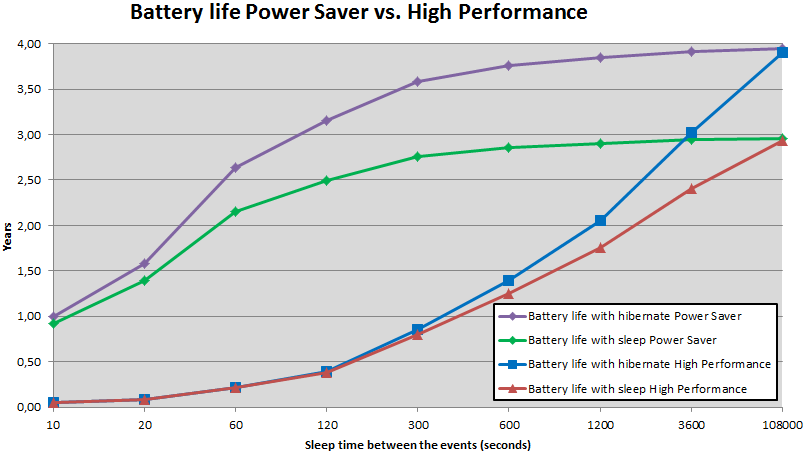
\includegraphics[height=8cm]{battery2}
%\rule{30em}{0.5pt}
\caption{Battery life High Performance vs. Power Saver}
\label{fig:batCalcPS}
\end{figure}
%-------------------------
\begin{figure}[htbp]
\centering
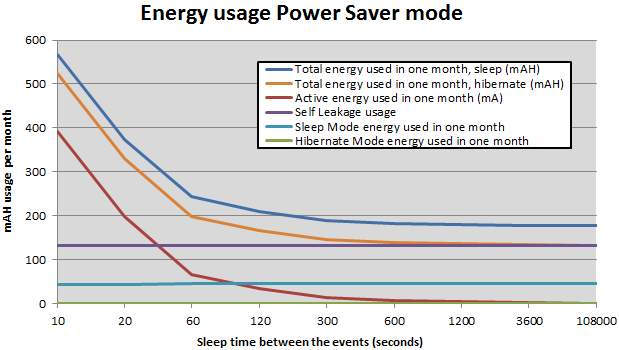
\includegraphics[height=8cm]{battery3}
\caption{Energy usage in Power Saver mode}
\label{fig:batCalcPS1}
\end{figure}
%--------------------------------
\begin{table}[!ht]
\begin{center}
\begin{tabular}{cc|c||c|c|l}
\cline{2-5}
 & \multicolumn{2}{ |c|| }{Deep Sleep} & \multicolumn{2}{c}{Hibernate}\vline\\ \cline{1-5}
\multicolumn{1}{ |c| }{Sleep duration} & High Performance & Power Saver & High Performance & Power Saver    \\ \cline{1-5}
\multicolumn{1}{ |c| }{10s} & 0,05 & 0,92 & 0,05 & 1,00    \\ %\cline{1-5}
\hline
\multicolumn{1}{ |c| }{1min} & 0,21 & 2,15 & 0,21 & 2,63   \\ %\cline{1-5}
\hline
\multicolumn{1}{ |c| }{3min} & 0,79 & 2,75 & 0,85 & 3,59   \\ %\cline{1-5}
\hline
\multicolumn{1}{ |c| }{10min} & 1,25 & 2,85 & 1,39 & 3,76   \\ %\cline{1-5}
\hline
\multicolumn{1}{ |c| }{20min} & 1,75 & 2,90 & 2,06 & 3,85  \\ %\cline{1-5}
\hline
\multicolumn{1}{ |c| }{1h} & 2,41 & 2,94 &3,02 & 3,91    \\ %\cline{1-5}
\hline
\multicolumn{1}{ |c| }{3h} & 2,94 & 2,96 &3,90 & 3,94    \\ %\cline{1-5}
\hline
%\multicolumn{1}{ |c  }{\multirow{2}{*}{Powers} } &
%\multicolumn{1}{ |c| }{gcd} & 2 & 2 & 0 & 0 & min \\ \cline{2-6}
%\multicolumn{1}{ |c  }{}                        &
%\multicolumn{1}{ |c| }{lcm} & 3 & 3 & 1 & 1 & max \\ \cline{1-6}
\end{tabular}
\caption{Battery life in years for High Performance and Power Saver}
\label{tab:cons2}
\end{center}
\end{table}
%-----------------------------
\begin{table}[!ht]
\begin{center}
\begin{tabular}[!ht]{|c|c|}
\hline
\textbf{Nr of samples per sensor} & \textbf{Average ON time (ms)}\\
\hline
10 & 210\\
\hline
3 & 194\\
\hline
\end{tabular}
\caption{Time needed to sample and store 4 sensors}
\label{tab:sendTime3}
\end{center}
\end{table}
\pagebreak
%-----------------------
\begin{figure}[htbp]
\centering
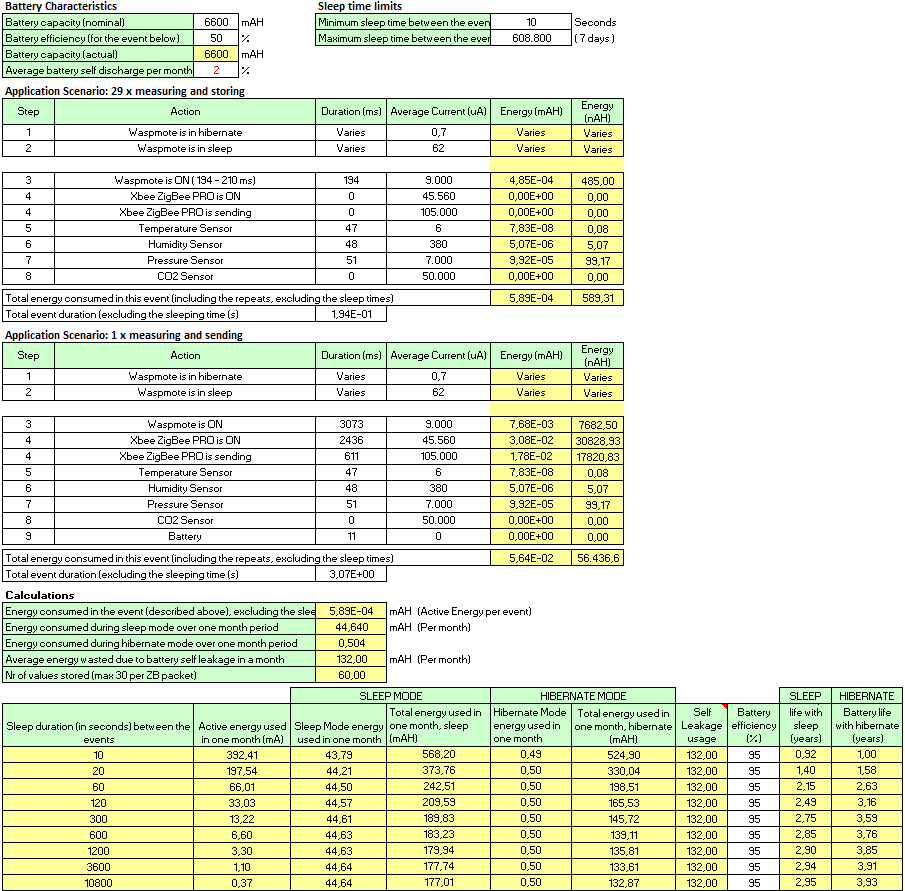
\includegraphics[height=18cm]{cons2}
\caption{Energy usage in High performance mode}
\label{fig:consump2}
\end{figure}
%-------------------------------------------------------------------
\clearpage
\pagebreak
\subsection{High Performance vs. Saver Mode, with ZigBee sleep}